% $Header: /cvsroot/latex-beamer/latex-beamer/solutions/generic-talks/generic-ornate-15min-45min.en.tex,v 1.5 2007/01/28 20:48:23 tantau Exp $

\documentclass{beamer}

\usepackage{caption}
\captionsetup{labelformat=empty,labelsep=none,font=scriptsize}
\setlength{\abovecaptionskip}{0pt}

\usepackage{color}
%% These definitions are based on darkred at
%% http://www.december.com/html/spec/colorcmyk.html
\definecolor{darkred}{cmyk}{0, 1, 1, 0.45}
\newcommand{\jul}{\textcolor{darkred}}
\newcommand{\jan}{\textcolor{blue}}

% This file is a solution template for:

% - Giving a talk on some subject.
% - The talk is between 15min and 45min long.
% - Style is ornate.



% Copyright 2004 by Till Tantau <tantau@users.sourceforge.net>.
%
% In principle, this file can be redistributed and/or modified under
% the terms of the GNU Public License, version 2.
%
% However, this file is supposed to be a template to be modified
% for your own needs. For this reason, if you use this file as a
% template and not specifically distribute it as part of a another
% package/program, I grant the extra permission to freely copy and
% modify this file as you see fit and even to delete this copyright
% notice. 


\mode<presentation>
{
  \usetheme{Warsaw}
  % or ...

  \setbeamercovered{transparent}
  % or whatever (possibly just delete it)
}


\usepackage[english]{babel}
% or whatever

\usepackage[latin1]{inputenc}
% or whatever

\usepackage{times}
\usepackage[T1]{fontenc}
% Or whatever. Note that the encoding and the font should match. If T1
% does not look nice, try deleting the line with the fontenc.


%% \title[Short Paper Title] % (optional, use only with long paper titles)
%% {Presentation Title}
%% \title[]{Initial findings}
%\subtitle {Eastern CASTNET sites, May-Sep.~2001} % (optional)

%% \author[Author, Another] % (optional, use only with lots of authors)
%% {F.~Author\inst{1} \and S.~Another\inst{2}}
%% % - Use the \inst{?} command only if the authors have different
%% %   affiliation.
%% \author[Swall et al.]{Jenise Swall\inst{1}, Ana Rappold\inst{2}, and Lucas Neas\inst{2}
% - Use the \inst{?} command only if the authors have different
%   affiliation.

%% \institute[Universities of Somewhere and Elsewhere] % (optional, but mostly needed)
%% {
%%   \inst{1}%
%%   Department of Computer Science\\
%%   University of Somewhere
%%   \and
%%   \inst{2}%
%%   Department of Theoretical Philosophy\\
%%   University of Elsewhere}
%% % - Use the \inst command only if there are several affiliations.
%% % - Keep it simple, no one is interested in your street address.
 %% \institute[VCU]
 %% {
 %%   \inst{1}%
 %%   Dept.\ of Statistical Sciences and Operations Research\\
 %%   Virginia Commonwealth University
 %%   \and
 %%   \inst{2}%
 %%   National Health and Environmental Effects Research Laboratory\\
 %%   U.S.~Environmental Protection Agency
 %% }

%% \date[Short Occasion] % (optional)
%% {Date / Occasion}
%% \date{Oct.\ 2017}

%% \subject{Talks}
% This is only inserted into the PDF information catalog. Can be left
% out. 



% If you have a file called "university-logo-filename.xxx", where xxx
% is a graphic format that can be processed by latex or pdflatex,
% resp., then you can add a logo as follows:

% \pgfdeclareimage[height=0.5cm]{university-logo}{university-logo-filename}
% \logo{\pgfuseimage{university-logo}}



% Delete this, if you do not want the table of contents to pop up at
% the beginning of each subsection:
\AtBeginSection[]
{
  \begin{frame}<beamer>{Outline}
    \tableofcontents[currentsection,currentsubsection]
  \end{frame}
}


% If you wish to uncover everything in a step-wise fashion, uncomment
% the following command: 

%\beamerdefaultoverlayspecification{<+->}

\useoutertheme{infolines}

\begin{document}

%% \begin{frame}
%%   \titlepage
%% \end{frame}

\begin{frame}{Outline}
  \tableofcontents
  % You might wish to add the option [pausesections]
\end{frame}


% Since this a solution template for a generic talk, very little can
% be said about how it should be structured. However, the talk length
% of between 15min and 45min and the theme suggest that you stick to
% the following rules:  

% - Exactly two or three sections (other than the summary).
% - At *most* three subsections per section.
% - Talk about 30s to 2min per frame. So there should be between about
%   15 and 30 frames, all told.


%% %%%%%%%%%%%%%%%%%%%%%%%%%%%%%%%%%%%%%%%%%%%%%%%%%%%%%%%%%%



%% %%%%%%%%%%%%%%%%%%%%%%%%%%%%%
%% Introductory material
%% \section[Background]{Background ideas and info}
\section[Background]{Setup for random forest models and simulations}

\begin{frame}{About the data used}

{\footnotesize
  
\noindent We tried many different random forest models:
\begin{itemize}
\item Using family-level taxa alone
\item Using order-level taxa alone
\item Using phylum-level taxa alone
\item Using family, order, and phylum-level taxa combined
\end{itemize}

\vspace{0.1in}

\noindent Time scale:
\begin{itemize}
\item Tried models utilizing all 61 days of observations in the data setthe time steps in the data
\item Tried models utilizing the first 15 days of observations. (After
  15 days, the observations are approx.~weekly, rather than every 2
  days.)
\end{itemize}
}

\end{frame}



\begin{frame}{Distribution of the degree days}

  {\scriptsize
  
    \noindent Since the degree days are so right-skewed, I also ran
    analyses using the square root of the degree days as the response
    variable.

    
\begin{figure}
  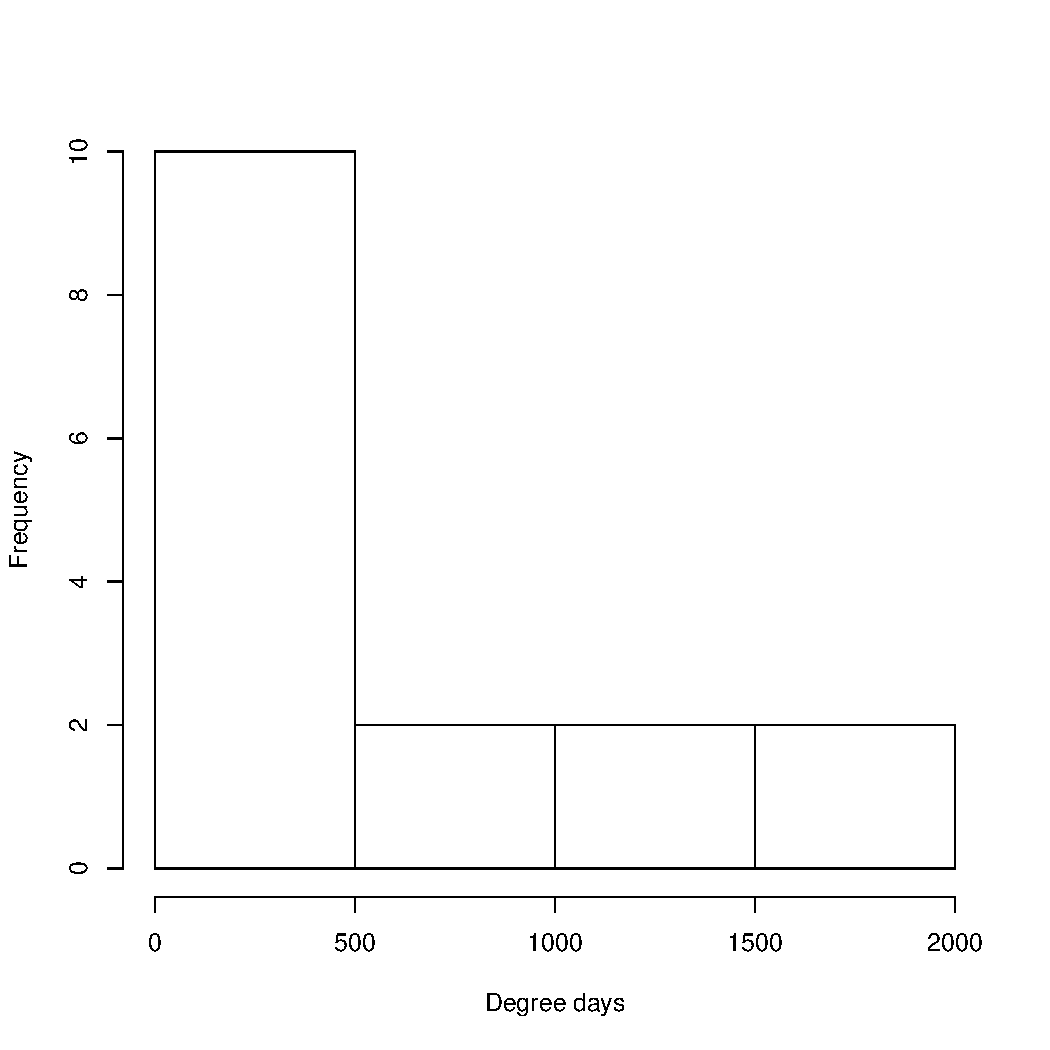
\includegraphics[width=2.1in]{degdays_all_time_steps_hist}
  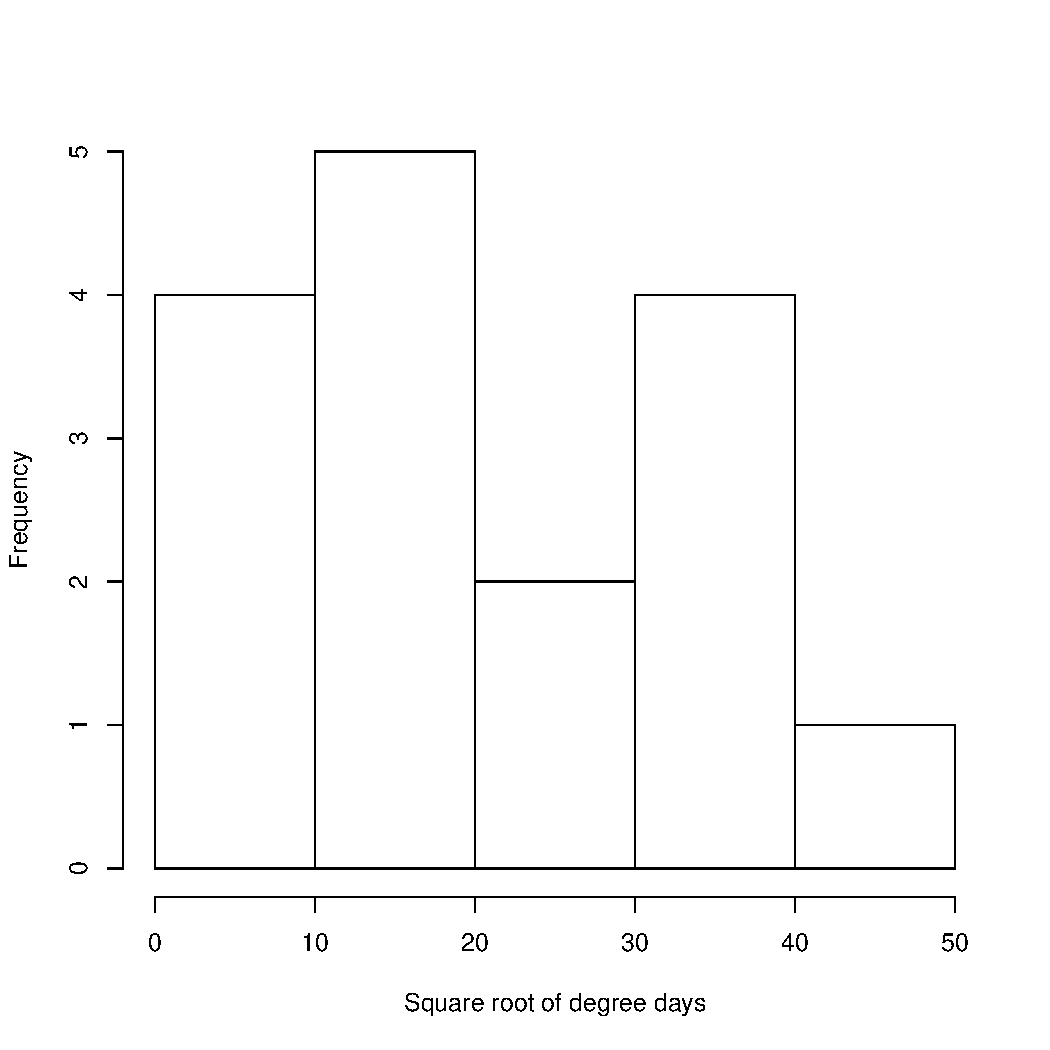
\includegraphics[width=2.1in]{sqrt_degdays_all_time_steps_hist}
\end{figure}
  }
  
\end{frame}



\begin{frame}{Looking at just the first 2 weeks}

  {\scriptsize
    \noindent After 15 days, the observations occur much less frequently, on the order of about once a week, making the distribution less skewed.
    
\begin{figure}
  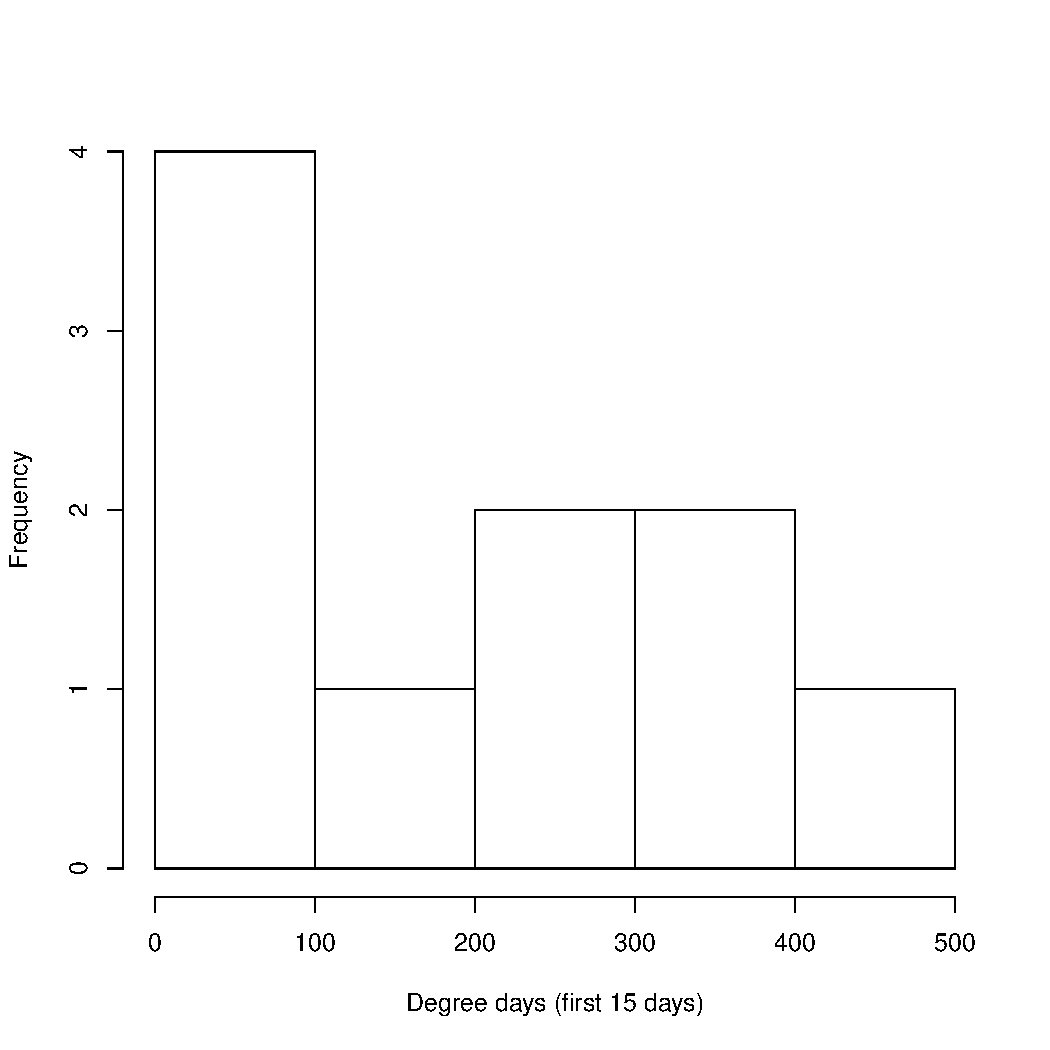
\includegraphics[width=2.1in]{degdays_first_two_weeks_hist}
  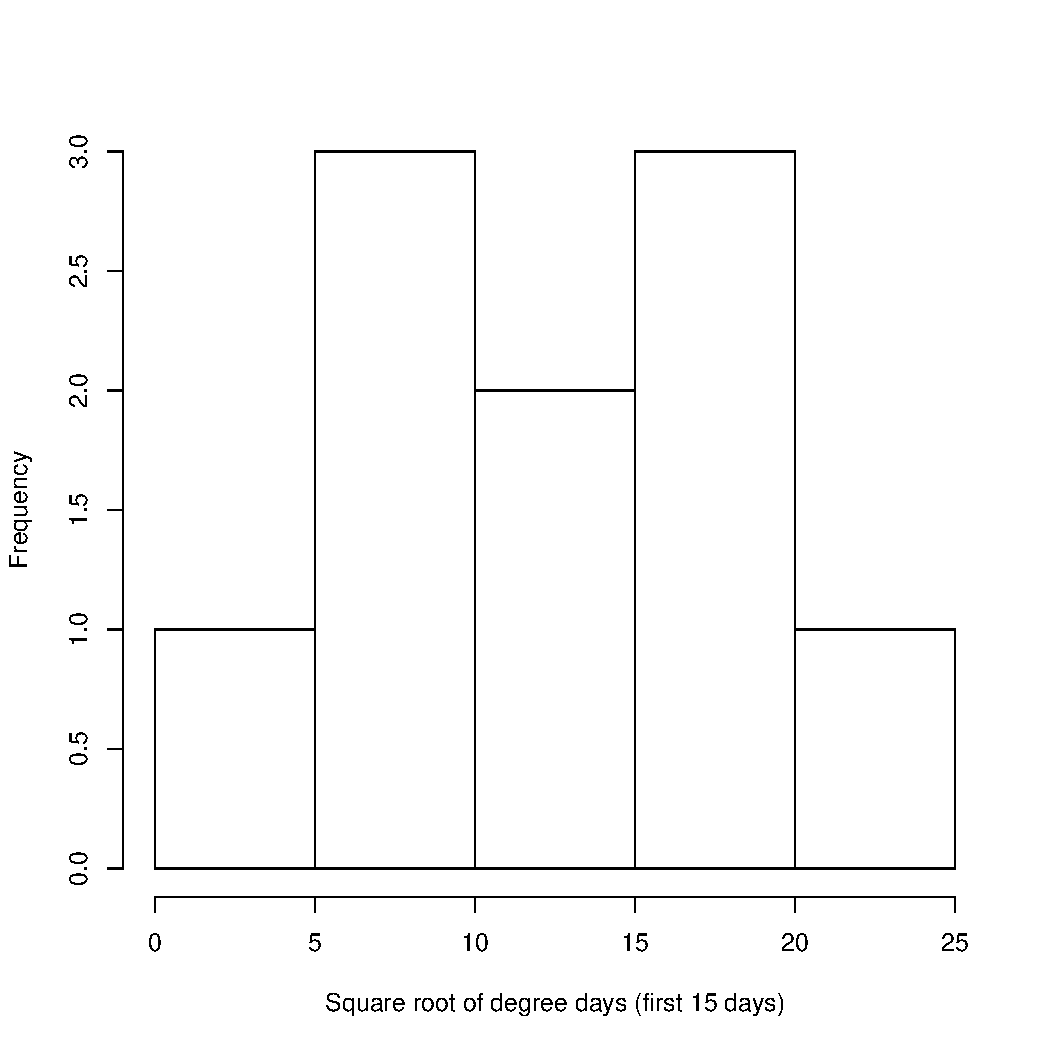
\includegraphics[width=2.1in]{sqrt_degdays_first_two_weeks_hist}
\end{figure}
  }
  
\end{frame}
%% %%%%%%%%%%%%%%%%%%%%%%%%%%%%%



%% %%%%%%%%%%%%%%%%%%%%%%%%%%%%%
\section[All time steps]{Using all time steps}


\begin{frame}{Using family taxa - original units}

  {\scriptsize
    
  \noindent Using original units:\\
  RMSE: 267.03  \hspace{0.05in}  Explained variation: 76.86\%

  \begin{center}
    \begin{figure}
      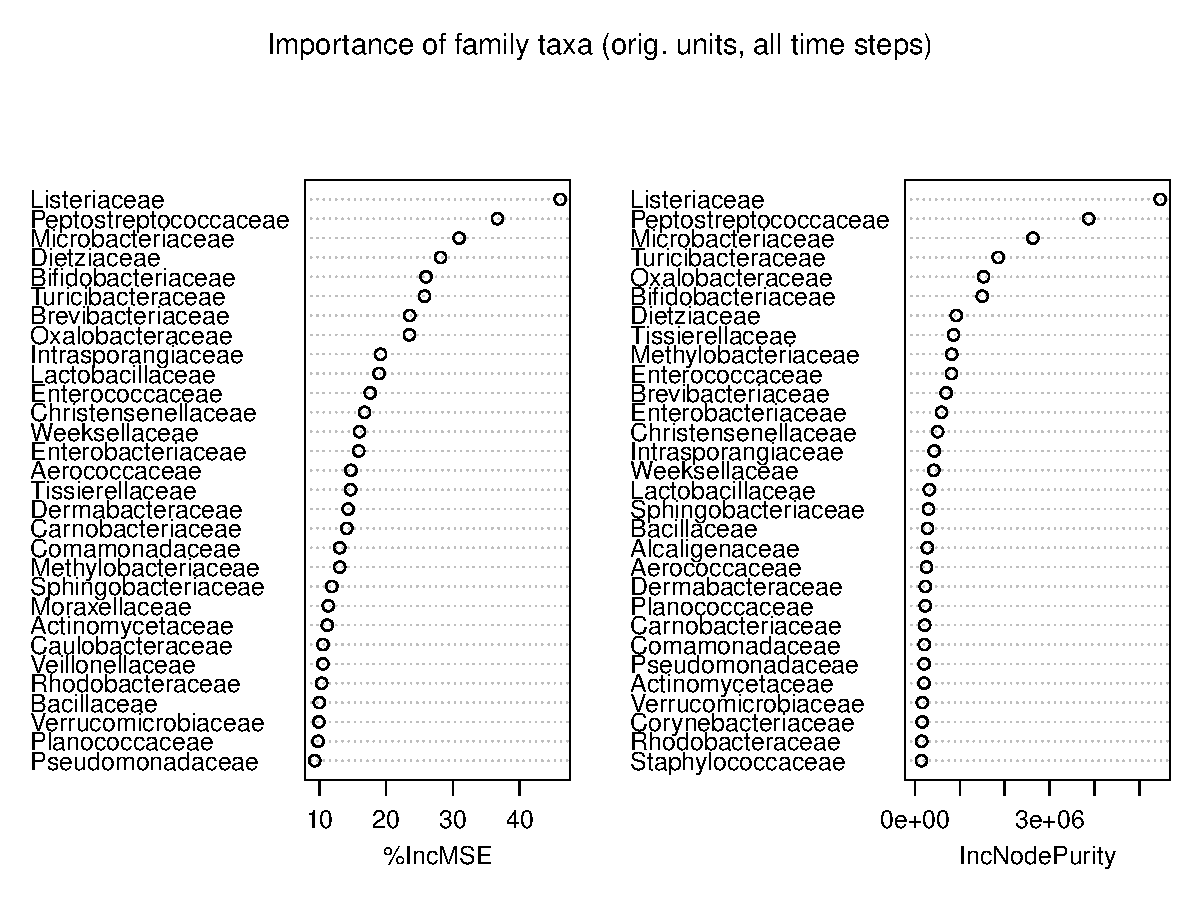
\includegraphics[width=3.25in]{../only_families/all_time_steps/orig_units_all_data_families_imp_plot}
    \end{figure}
  \end{center}
  \vspace{-0.25in}

\noindent There are 51 family-level taxa which were considered as predictors.
}

\end{frame}



\begin{frame}{Using family taxa - sqrt transformation}

  {\scriptsize
    
  \noindent Using square root transformation:\\
  RMSE: 5.64  \hspace{0.05in}  Explained variation: 79.43\%

  \vspace{0.05in}
  
  \noindent If you transform the predictions back to the original
  scale and then compare with the original degree days, the RMSE is
  approximately 296.89.
  
\begin{center}
\begin{figure}
  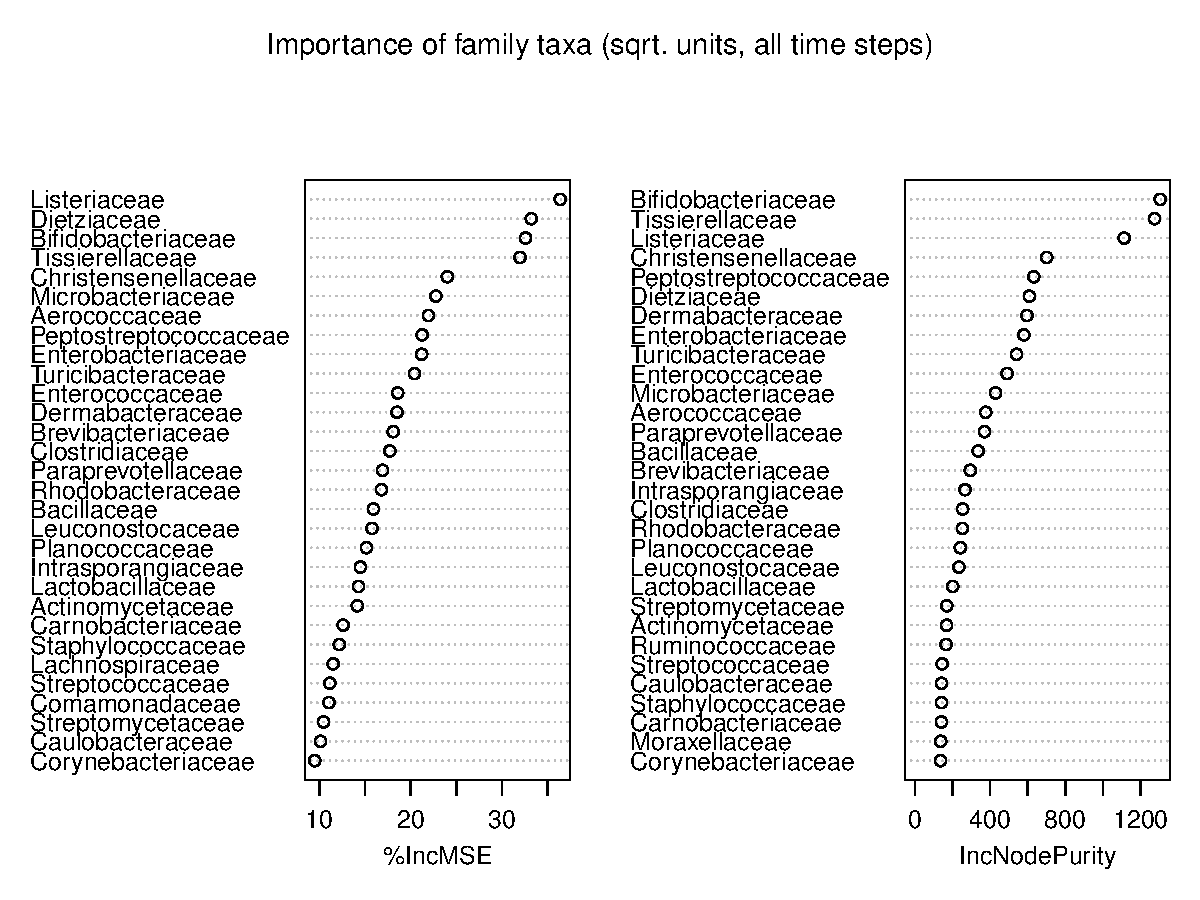
\includegraphics[width=3.25in]{../only_families/all_time_steps/sqrt_units_all_data_families_imp_plot}
\end{figure}
\end{center}
\vspace{-0.25in}
}
  
\end{frame}



\begin{frame}{Using order taxa - original units}

  {\scriptsize
    
  \noindent Using original units:\\
  RMSE: 281.16  \hspace{0.05in}  Explained variation: 74.35\%

  \begin{center}
    \begin{figure}
      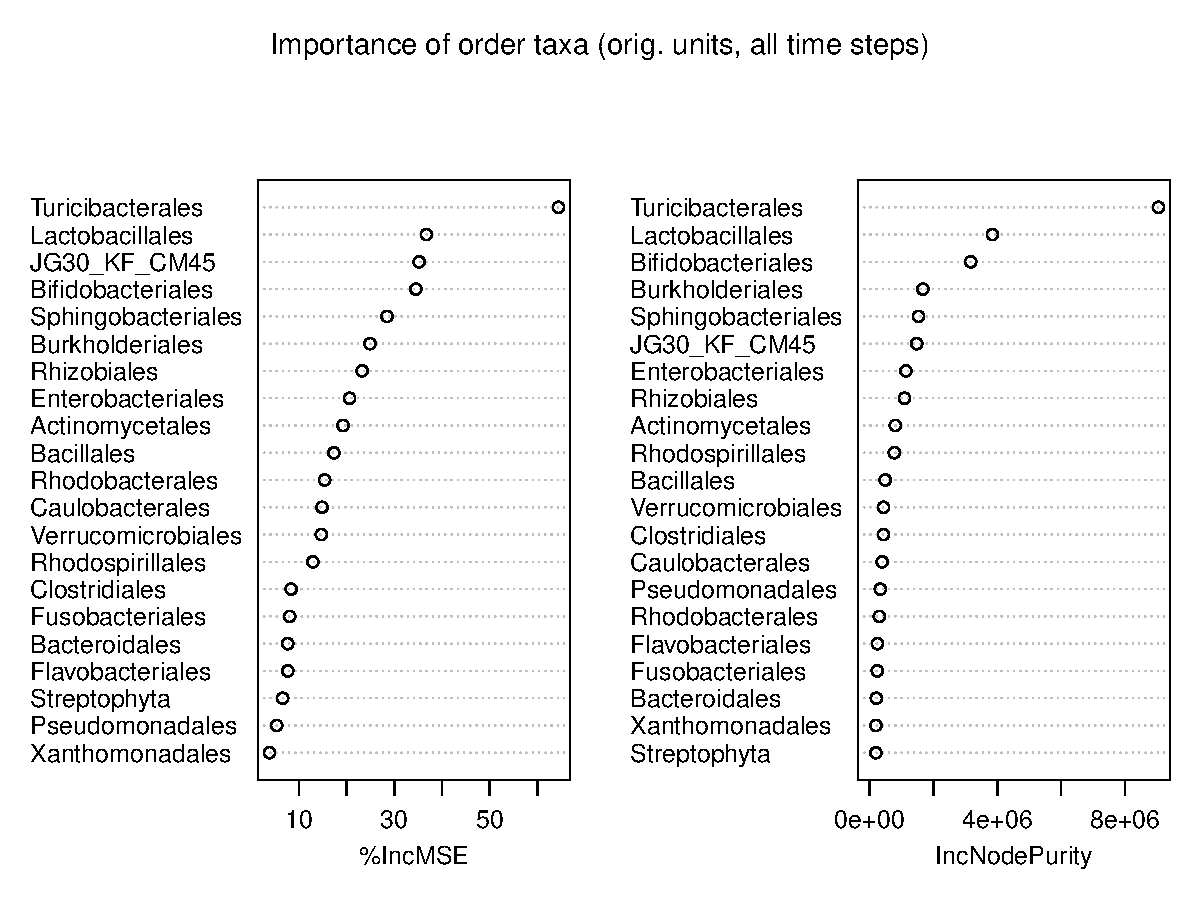
\includegraphics[width=3.25in]{../only_orders/all_time_steps/orig_units_all_data_orders_imp_plot}
    \end{figure}
  \end{center}
  \vspace{-0.25in}

\noindent There are 21 order-level taxa which were considered as predictors.
}

\end{frame}



\begin{frame}{Using order taxa - sqrt transformation}

  {\scriptsize
    
  \noindent Using square root transformation:\\
  RMSE: 5.40  \hspace{0.05in}  Explained variation: 81.14\%

  \vspace{0.05in}
  
  \noindent If you transform the predictions back to the original
  scale and then compare with the original degree days, the RMSE is
  approximately 289.65.
  
\begin{center}
\begin{figure}
  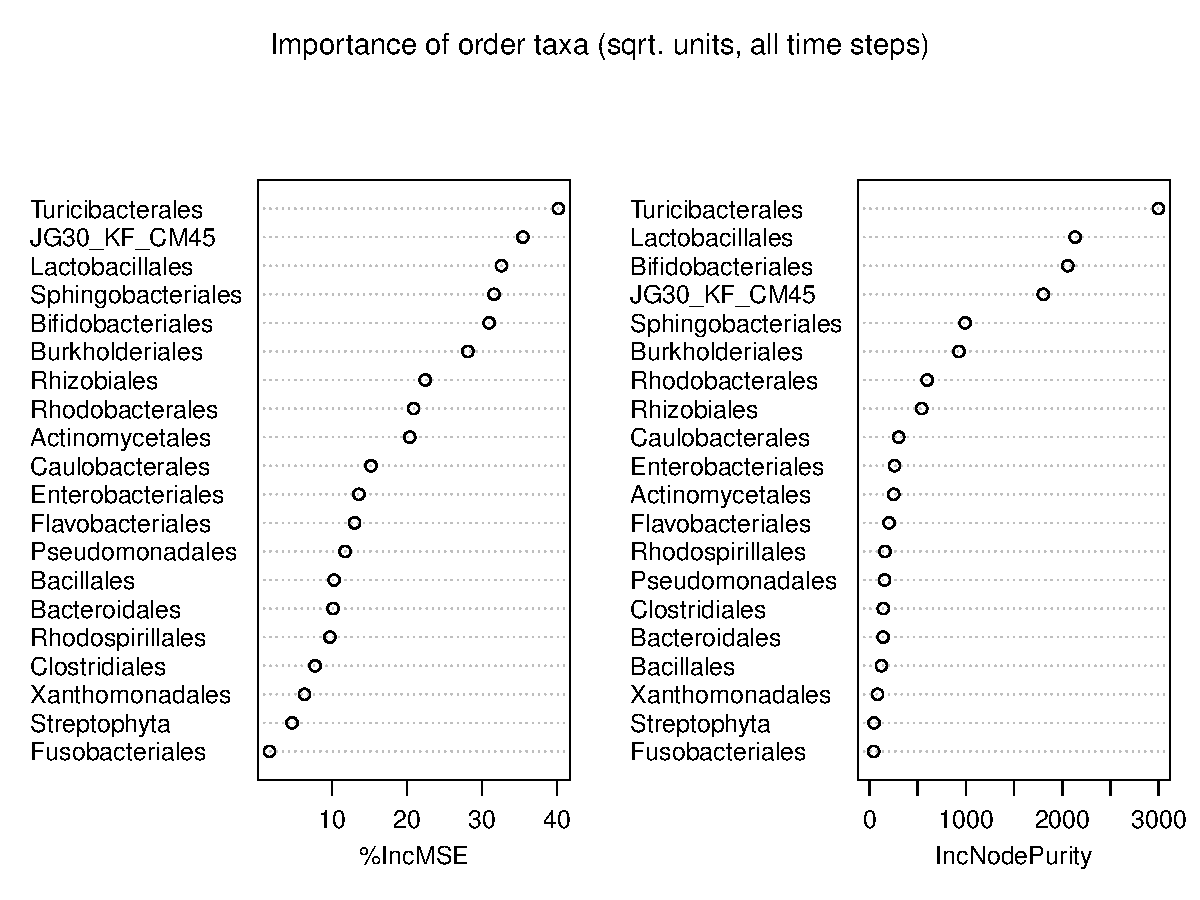
\includegraphics[width=3.25in]{../only_orders/all_time_steps/sqrt_units_all_data_orders_imp_plot}
\end{figure}
\end{center}
\vspace{-0.25in}
}
  
\end{frame}



\begin{frame}{Using combined taxa - original units}

  {\scriptsize
    
  \noindent Using original units:\\
  RMSE: 247.60  \hspace{0.05in}  Explained variation: 80.10\%

  \begin{center}
    \begin{figure}
      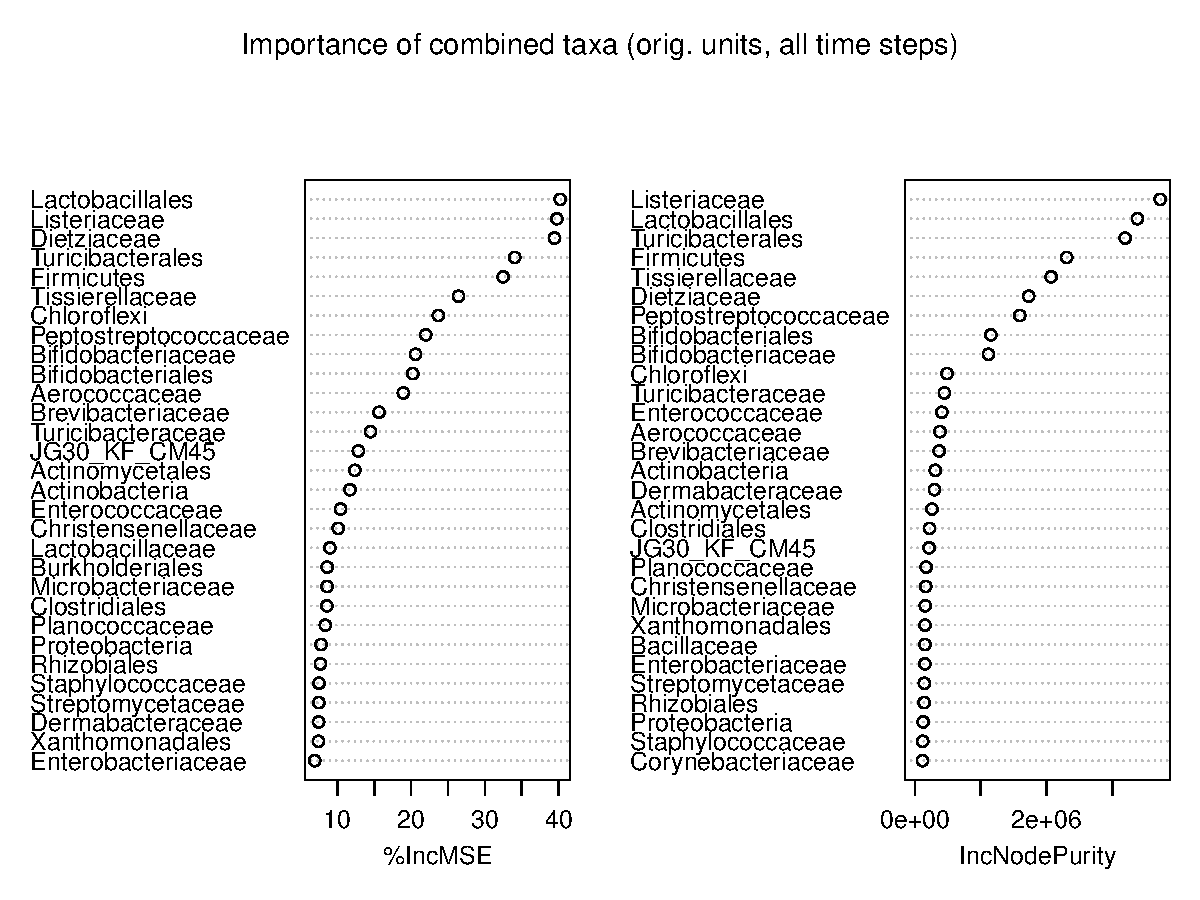
\includegraphics[width=3.25in]{../all_together/all_time_steps/orig_units_all_data_combined_imp_plot}
    \end{figure}
  \end{center}
  \vspace{-0.25in}

\noindent There are 82 taxa which were considered as predictors.
}

\end{frame}



\begin{frame}{Using combined taxa - sqrt transformation}

  {\scriptsize
    
  \noindent Using square root transformation:\\
  RMSE: 4.91  \hspace{0.05in}  Explained variation: 84.39\%

  \vspace{0.05in}
  
  \noindent If you transform the predictions back to the original
  scale and then compare with the original degree days, the RMSE is
  approximately 262.65.
  
\begin{center}
\begin{figure}
  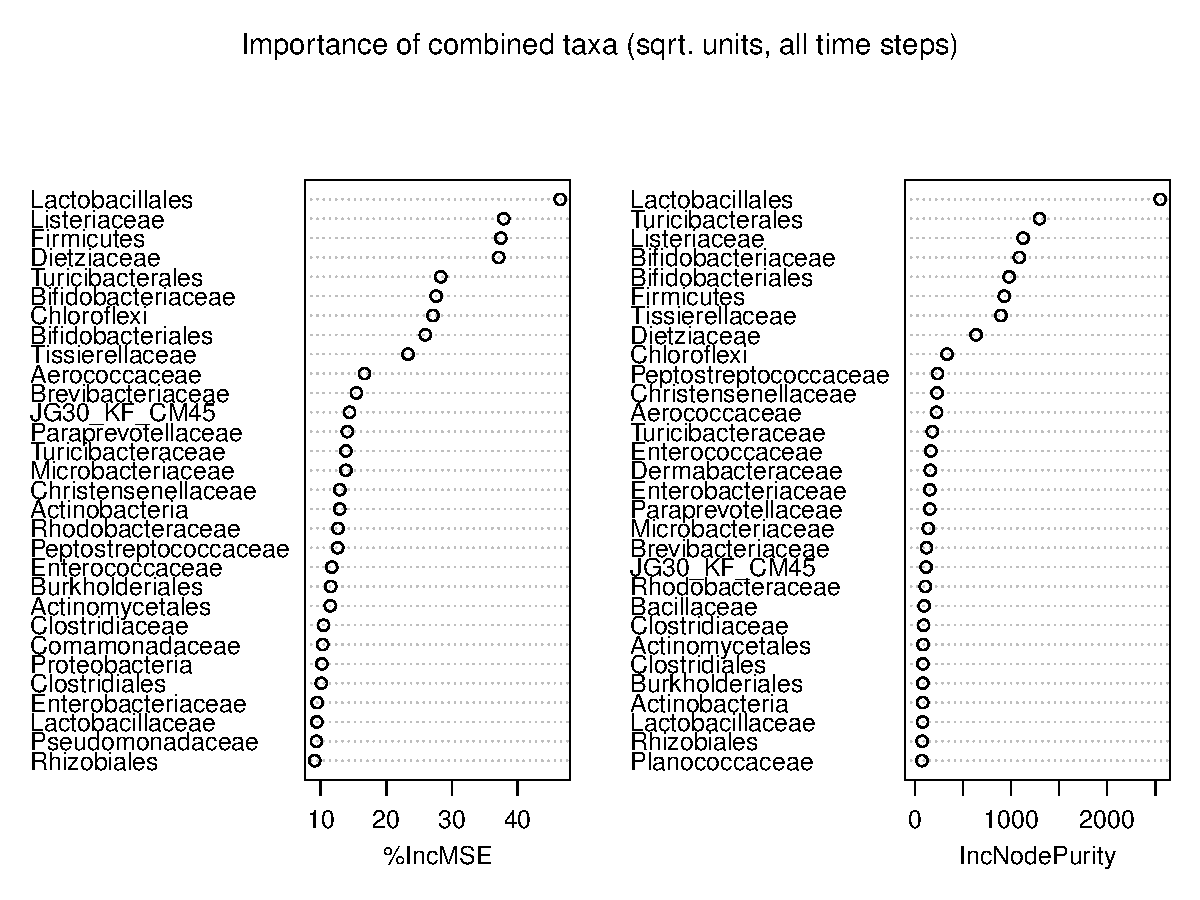
\includegraphics[width=3.25in]{../all_together/all_time_steps/sqrt_units_all_data_combined_imp_plot}
\end{figure}
\end{center}
\vspace{-0.25in}
}
  
\end{frame}
%% %%%%%%%%%%%%%%%%%%%%%%%%%%%%%




%% %%%%%%%%%%%%%%%%%%%%%%%%%%%%%
\section[First 15 days]{Using first 15 days}


\begin{frame}{Using family taxa - original units}

  {\scriptsize
    
  \noindent Using original units:\\
  RMSE: 84.19  \hspace{0.05in}  Explained variation: 69.76\%

  \begin{center}
    \begin{figure}
      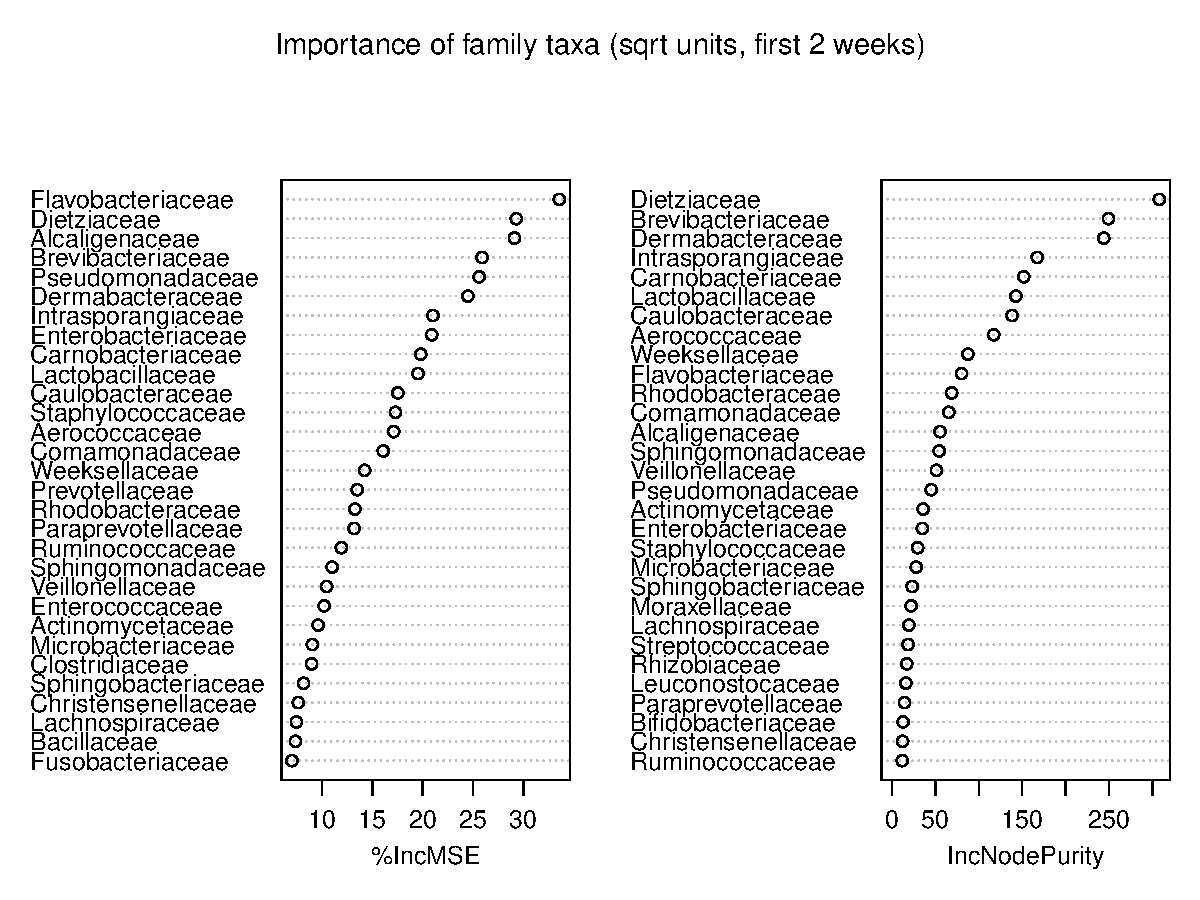
\includegraphics[width=3.25in]{../only_families/first_two_weeks/sqrt_units_first_two_weeks_families_imp_plot}
    \end{figure}
  \end{center}
  \vspace{-0.25in}

\noindent Remember, there are 51 family-level taxa which were
considered as predictors.
}

\end{frame}



\begin{frame}{Using family taxa - sqrt transformation}

  {\scriptsize
    
  \noindent Using square root transformation:\\
  RMSE: 3.06  \hspace{0.05in}  Explained variation: 78.65\%

  \vspace{0.05in}
  
  \noindent If you transform the predictions back to the original
  scale and then compare with the original degree days, the RMSE is
  approximately 91.35.
  
\begin{center}
\begin{figure}
  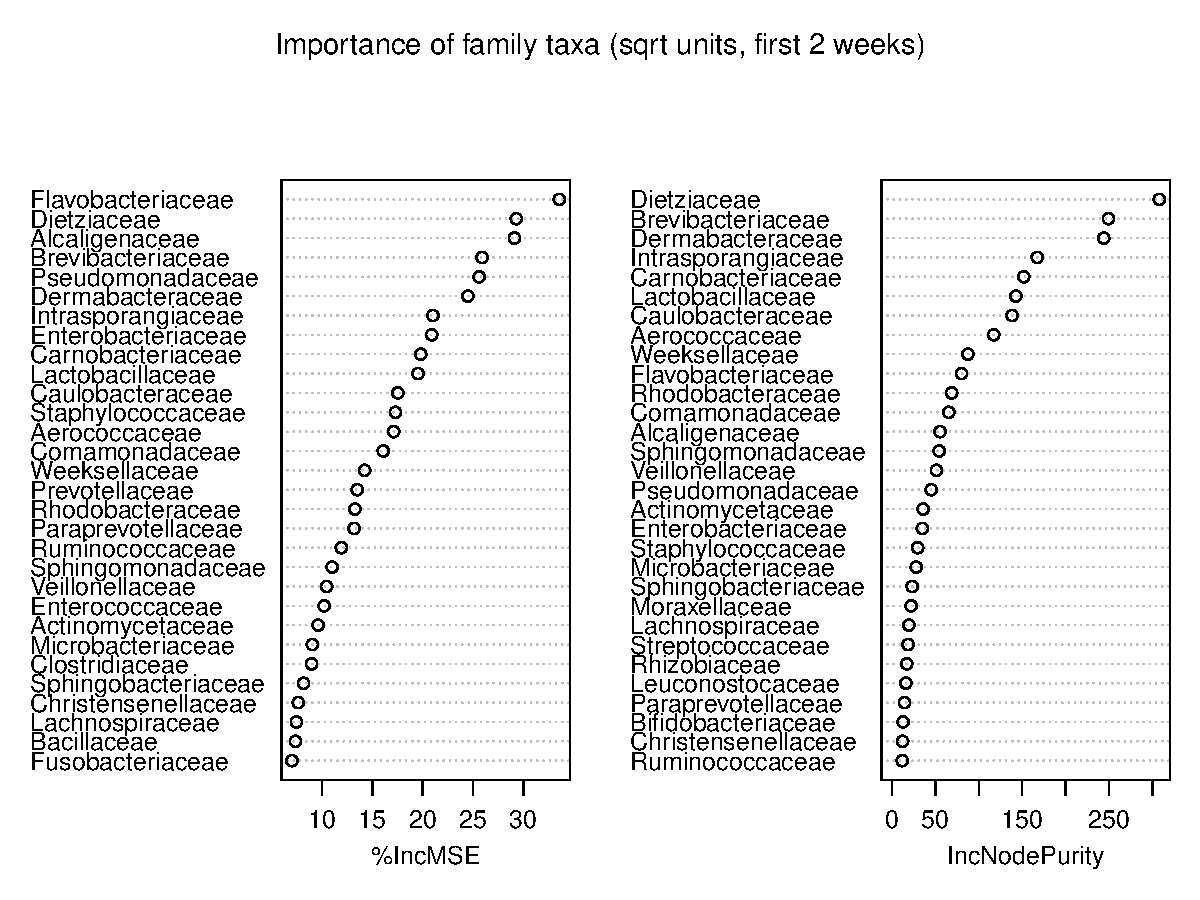
\includegraphics[width=3.25in]{../only_families/first_two_weeks/sqrt_units_first_two_weeks_families_imp_plot}
\end{figure}
\end{center}
\vspace{-0.25in}
}
  
\end{frame}



\begin{frame}{Using order taxa - original units}

  {\scriptsize
    
  \noindent Using original units:\\
  RMSE: 69.02  \hspace{0.05in}  Explained variation: 79.68\%

  \begin{center}
    \begin{figure}
      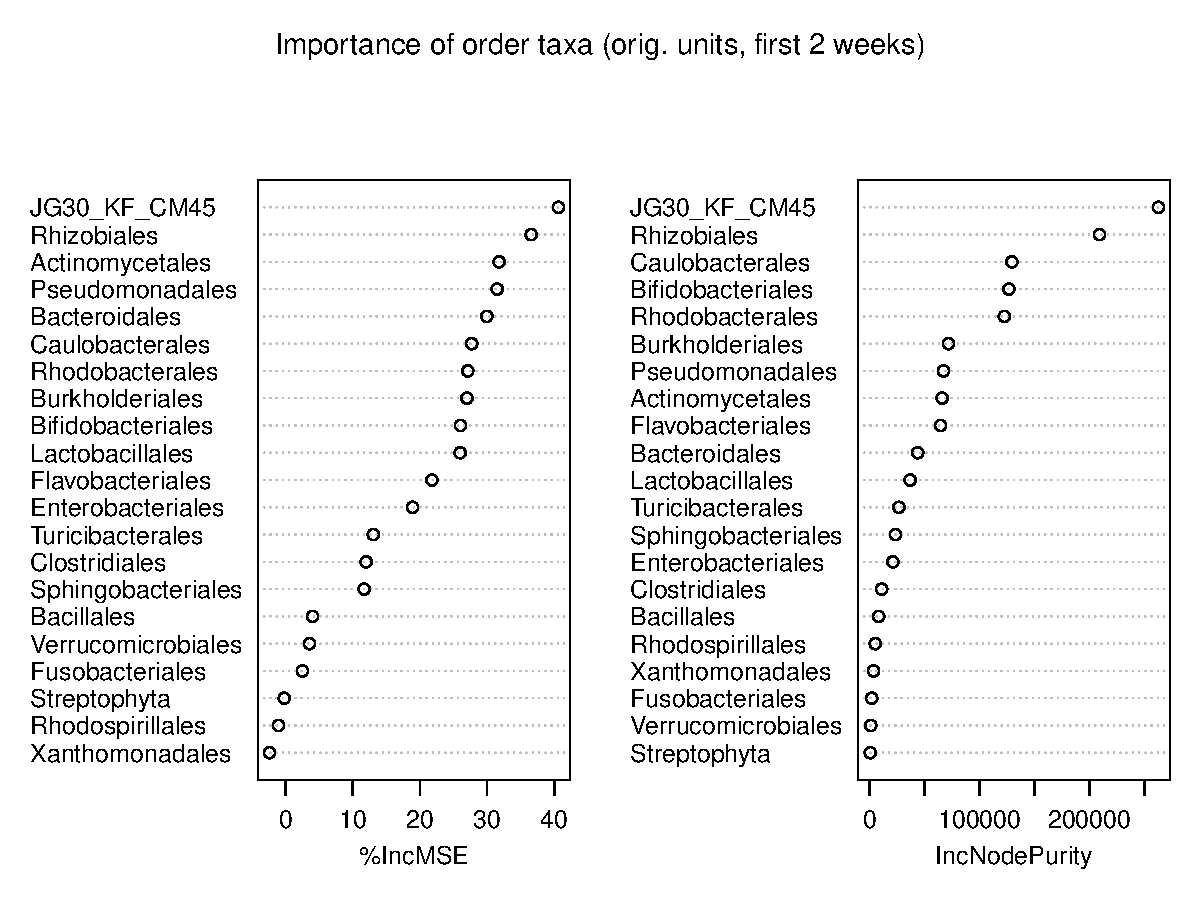
\includegraphics[width=3.25in]{../only_orders/first_two_weeks/orig_units_first_two_weeks_orders_imp_plot}
    \end{figure}
  \end{center}
  \vspace{-0.25in}

\noindent Remember, there are 21 order-level taxa which were considered as predictors.
}

\end{frame}



\begin{frame}{Using order taxa - sqrt transformation}

  {\scriptsize
    
  \noindent Using square root transformation:\\
  RMSE: 2.93  \hspace{0.05in}  Explained variation: 80.50\%

  \vspace{0.05in}
  
  \noindent If you transform the predictions back to the original
  scale and then compare with the original degree days, the RMSE is
  approximately 83.05.
  
\begin{center}
\begin{figure}
  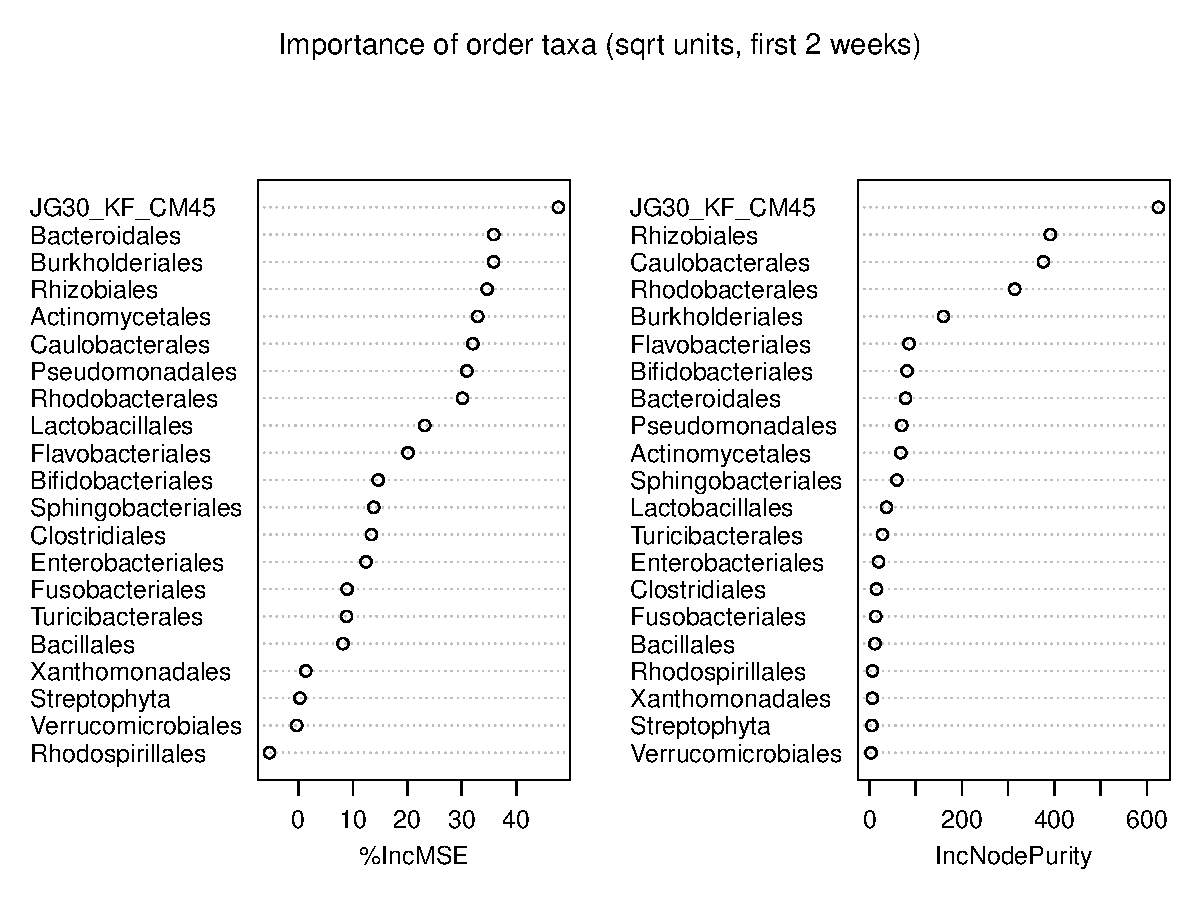
\includegraphics[width=3.25in]{../only_orders/first_two_weeks/sqrt_units_first_two_weeks_orders_imp_plot}
\end{figure}
\end{center}
\vspace{-0.25in}
}
  
\end{frame}



\begin{frame}{Using combined taxa - original units}

  {\scriptsize
    
  \noindent Using original units:\\
  RMSE: 69.07  \hspace{0.05in}  Explained variation: 79.65\%

  \begin{center}
    \begin{figure}
      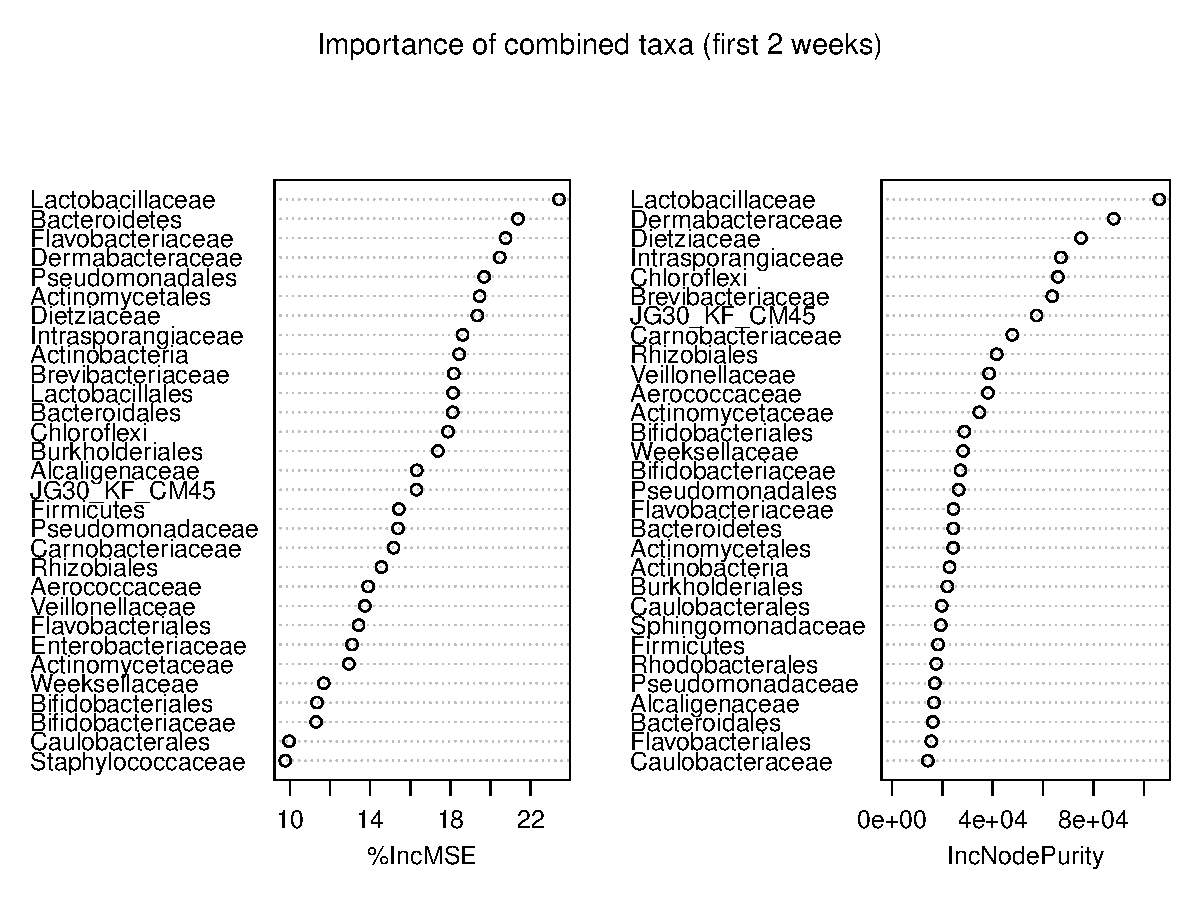
\includegraphics[width=3.25in]{../all_together/first_two_weeks/orig_units_first_two_weeks_combined_imp_plot}
    \end{figure}
  \end{center}
  \vspace{-0.25in}

\noindent Remember, there are 82 taxa which were considered as predictors.
}

\end{frame}



\begin{frame}{Using combined taxa - sqrt transformation}

  {\scriptsize
    
  \noindent Using square root transformation:\\
  RMSE: 2.76  \hspace{0.05in}  Explained variation: 82.69\%

  \vspace{0.05in}
  
  \noindent If you transform the predictions back to the original
  scale and then compare with the original degree days, the RMSE is
  approximately 77.97.
  
\begin{center}
\begin{figure}
  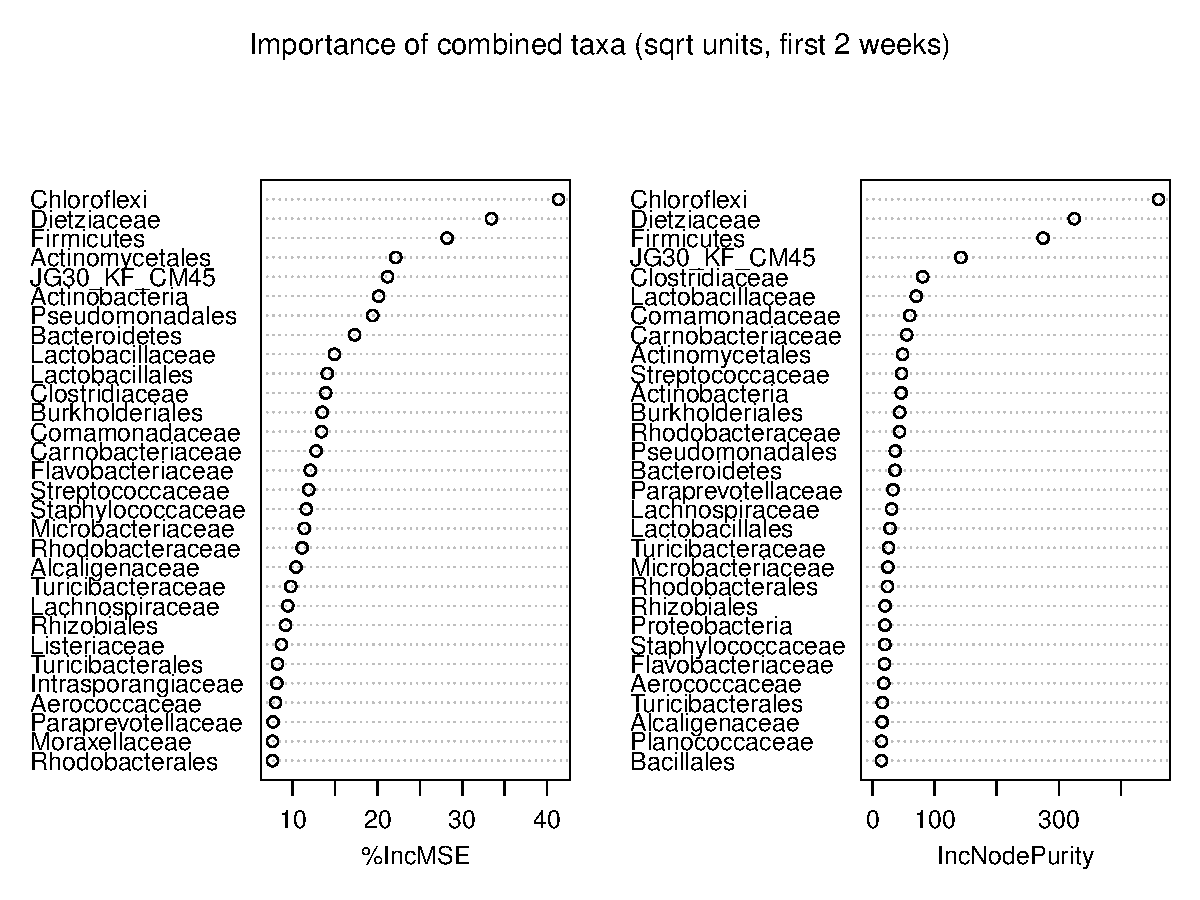
\includegraphics[width=3.25in]{../all_together/first_two_weeks/sqrt_units_first_two_weeks_combined_imp_plot}
\end{figure}
\end{center}
\vspace{-0.25in}
}
  
\end{frame}



\end{document}








\begin{frame}{``Common'' phylum taxa}

\begin{itemize}
\item Actinobacteria
\item Bacteroidetes
\item Firmicutes
\item Proteobacteria
\item All others grouped together as ``rare''
\end{itemize}

\vspace{0.05in}

\noindent These phyla are consistent with Pechal et al (2013).  See
their Figure 1a.

\end{frame}




\begin{frame}{``Common'' order taxa}

\noindent For order taxa, it's not clear which taxa should be
considered ``rare''.  Depending on whether you look at relative
abundance overall, by day, or by day-subject, you'll get different
numbers of ``common'' (not rare) taxa.
  
\begin{itemize}
\item There are only 6 taxa which have more than 3\% of overall
  relative abundance.  This seems too few and would leave out taxa
  which are prevalent for only a short time.
\item There are 13 taxa which have more than 3\% relative abundance on
  at least one day for at least one cadaver.  This list may be too
  broad, including taxa that are prevalent on just 1-2 cadavers for a
  short period of time.
\end{itemize}

\vspace{0.05in}

\noindent I've taken the middle path, including taxa with have 3\%
relative abundance (over all cadavers) for at least one day.  This
leaves 11 taxa.

\end{frame}




\begin{frame}{``Common'' family taxa}

\noindent For family taxa, the situation is similar to that for the order taxa.
  
\begin{itemize}
\item There are only 8 taxa which have more than 3\% of overall
  relative abundance.  This seems too few and would leave out taxa
  which are prevalent for only a short time.
\item There are 32 taxa which have more than 3\% relative abundance on
  at least one day for at least one cadaver.  This list may be too
  broad, including taxa that are prevalent on just 1-2 cadavers for a
  short period of time.
\end{itemize}

\vspace{0.05in}

\noindent Again, I've taken the middle path, including taxa which have
3\% relative abundance (over all cadavers) for at least one day.  This
leaves 19 taxa, which is similar to the number of taxa represented in
Figure 1b of Pechal et al (2013).

\end{frame}
%% %%%%%%%%%%%%%%%%%%%%%%%%%%%%%




%% %%%%%%%%%%%%%%%%%%%%%%%%%%%%%
\section[Graphics]{Exploratory graphics}

\begin{frame}{Variability in taxa counts between individuals}

\begin{center}
\begin{figure}
  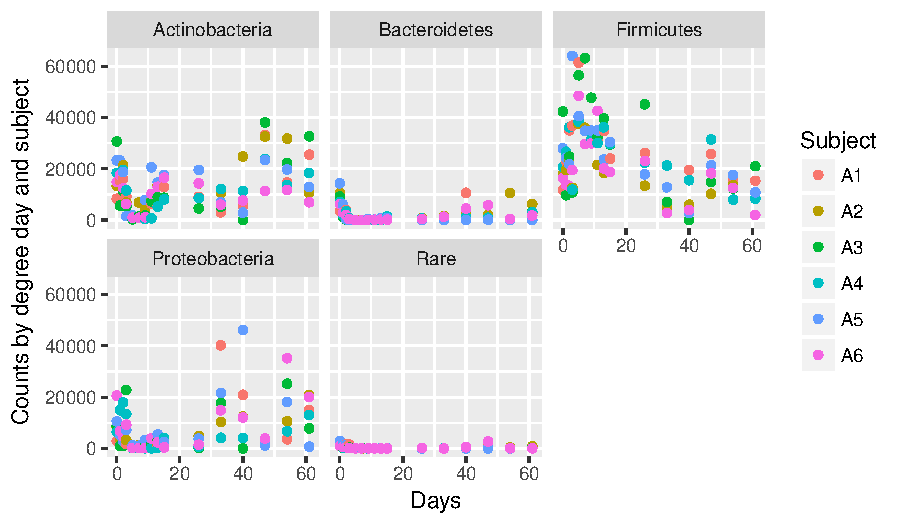
\includegraphics[width=4.5in]{phyla_scatter_counts_by_day_bacteria}
\end{figure}
\end{center}
\vspace{-0.05in}
\noindent {\scriptsize There is extensive variability in phyla counts
  between cadavers.  The same is true for orders and families.}

\end{frame}




\begin{frame}{First 5 days: compare subjects}

\begin{center}
\begin{figure}
  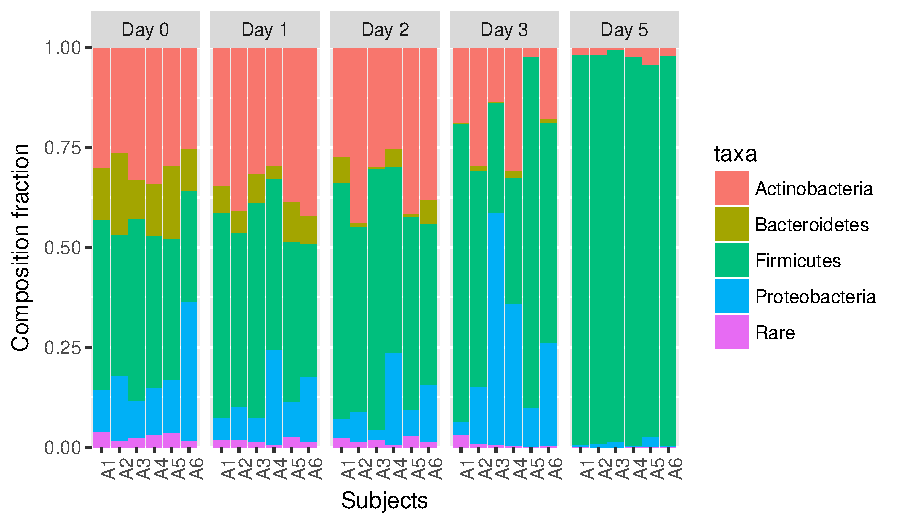
\includegraphics[width=4.5in]{phyla_first5_frac_bars_by_day_indiv}
\end{figure}
\end{center}
\vspace{-0.05in}
\noindent {\scriptsize There is some variability between cadavers, even when looking at fractions, rather than counts.  This graph shows phyla, but there is similar variability for orders and families.}

\end{frame}




\begin{frame}{First 5 days: average fractional composition (phyla)}

\begin{center}
\begin{figure}
  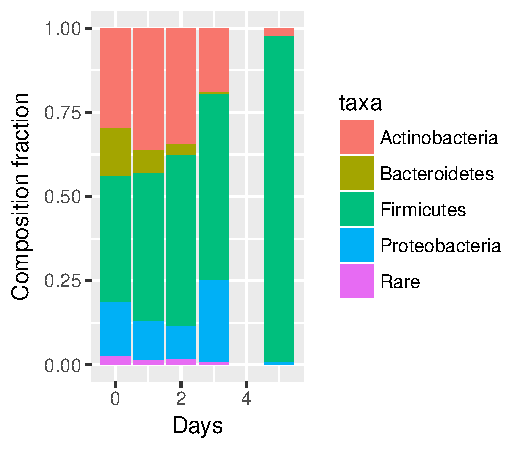
\includegraphics[width=2.5in]{phyla_first5_avgfrac_bars_by_day}
\end{figure}
\end{center}
\vspace{-0.05in}
\noindent {\scriptsize Comparing with Pechal et al (2013), Fig.~1a, our graph has less Proteobacteria and more Actinobacteria.}

\end{frame}



%% There were too many taxa to fit on this graph!
%% \begin{frame}{First 5 days: average fractional composition (families)}

%% \begin{center}
%% \begin{figure}
%%   \includegraphics[width=2.0in]{families_first5_avgfrac_bars_by_day}
%% \end{figure}
%% \end{center}
%% \vspace{-0.05in}
%% \noindent {\scriptsize Compare with Pechal et al (2013), Fig.~1b.  Our dataset indicates the presence of some families not present in their graph, and vice-versa.}

%% \end{frame}



\begin{frame}{Taxa patterns by degree days (phyla)}

\begin{center}
\begin{figure}
  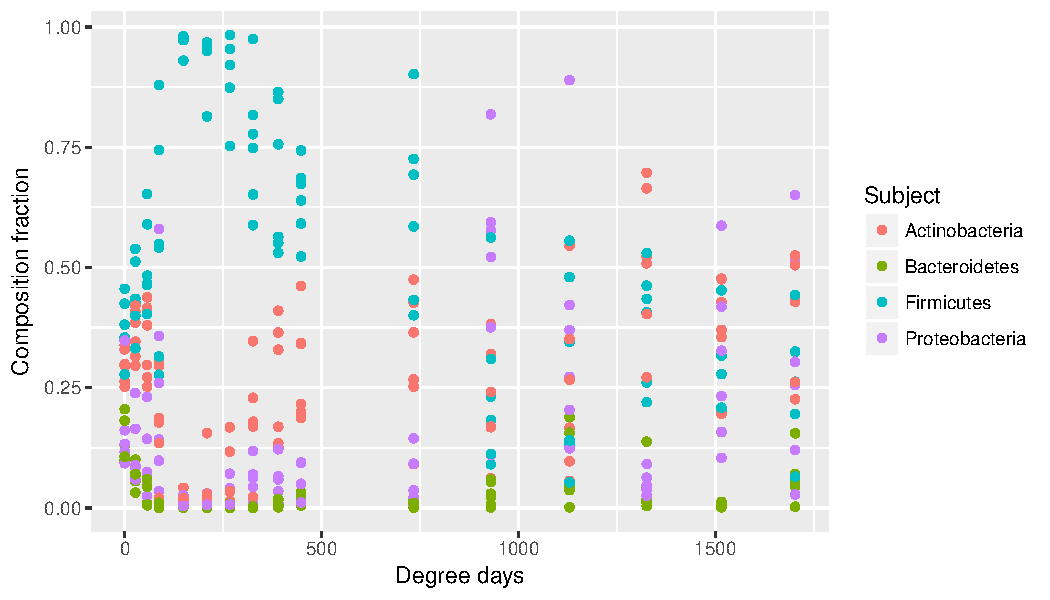
\includegraphics[width=4.5in]{phyla_scatter_frac_by_degday}
\end{figure}
\end{center}
\vspace{-0.1in}
\noindent {\scriptsize Individual cadavers are not distinguished in this graph.}

\end{frame}



\begin{frame}{Taxa patterns by degree days (orders)}

\begin{center}
\begin{figure}
  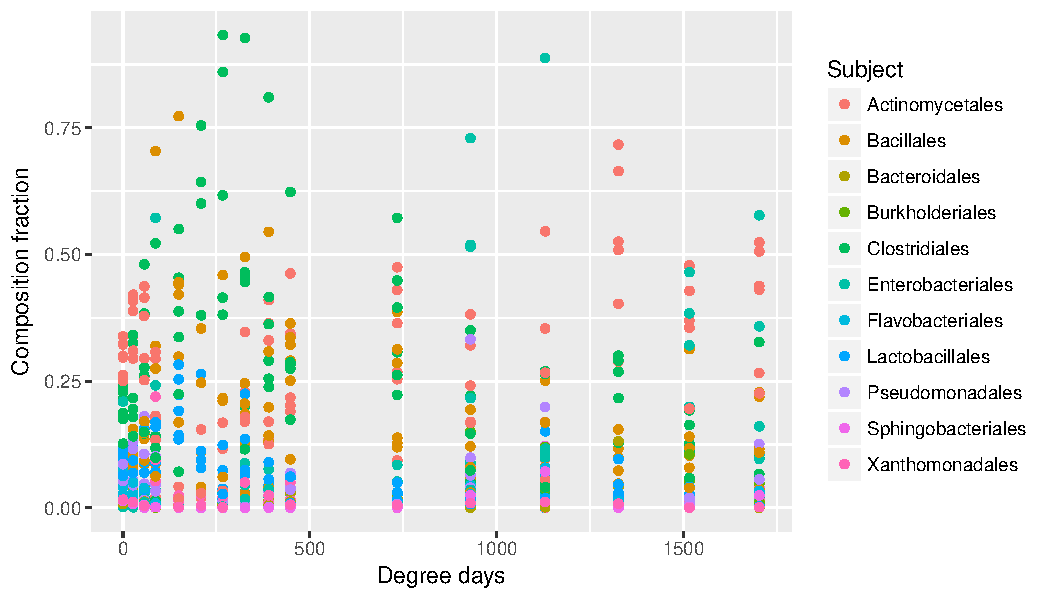
\includegraphics[width=4.5in]{orders_scatter_frac_by_degday}
\end{figure}
\end{center}
\vspace{-0.1in}
\noindent {\scriptsize Individual cadavers are not distinguished in this graph.}

\end{frame}



\begin{frame}{Taxa patterns by degree days (families)}

\begin{center}
\begin{figure}
  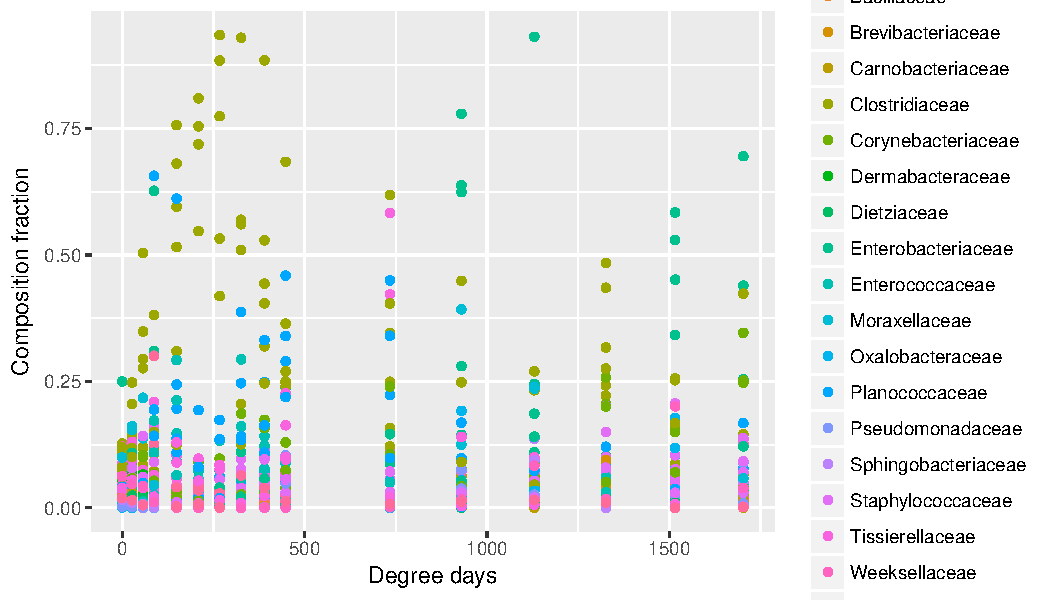
\includegraphics[width=4.5in]{families_scatter_frac_by_degday}
\end{figure}
\end{center}
\vspace{-0.1in}
\noindent {\scriptsize There are too many family-level taxa to display their names properly in the figure.}

\end{frame}
%% %%%%%%%%%%%%%%%%%%%%%%%%%%%%%




%% %%%%%%%%%%%%%%%%%%%%%%%%%%%%%
\section{Analysis ideas}


\begin{frame}{Issues/discussion}
  
\begin{itemize}
\item The explanatory variables are compositional fractions (for each day and each cadaver).
\item Multicollinearity (strong dependencies among the explanatory variables) makes it difficult to use typical modeling techniques.
\item Metcalf et al used random forests to try to predict the PMI; this strategy can be efficient with multicollinearity.  That is the approach I've pursued in the next few slides.
  \item You had mentioned DFA (discriminant function analysis) in an earlier email.  That would involve treating the response variable not as a number of days (or degree days), but as a classification variable.  That changes how we would interpret the model.  I did do some runs with random forest models for classification (which would be similar), and we can talk more about those if you like.
\end{itemize}

\end{frame}




\begin{frame}{Random forests}

\begin{itemize}
\item I used days (PMI) as the
  response variable, rather than degree days.  However, these are
  strongly correlated in our example, so I expect that the results
  would be similar.
  \item Random forest models are a bit hard to interpret; the
    estimates are made based on an ensemble of decision trees.  This
    means that you can't write down the fitted model as an equation
    (as you would for, say, a linear regression model).  However, it
    is straightforward to use a fitted model to make predictions for a
    new set of data.
\item Like Metcalf et al, I used cross-validation to estimate the
  best parameters for the random forest model.  These parameters are
  the number of variables considered at each split of the tree and the
  number of trees making up your ensemble.
\end{itemize}

\end{frame}


  

\begin{frame}{Fitting the order taxa}

\begin{center}
\begin{figure}
  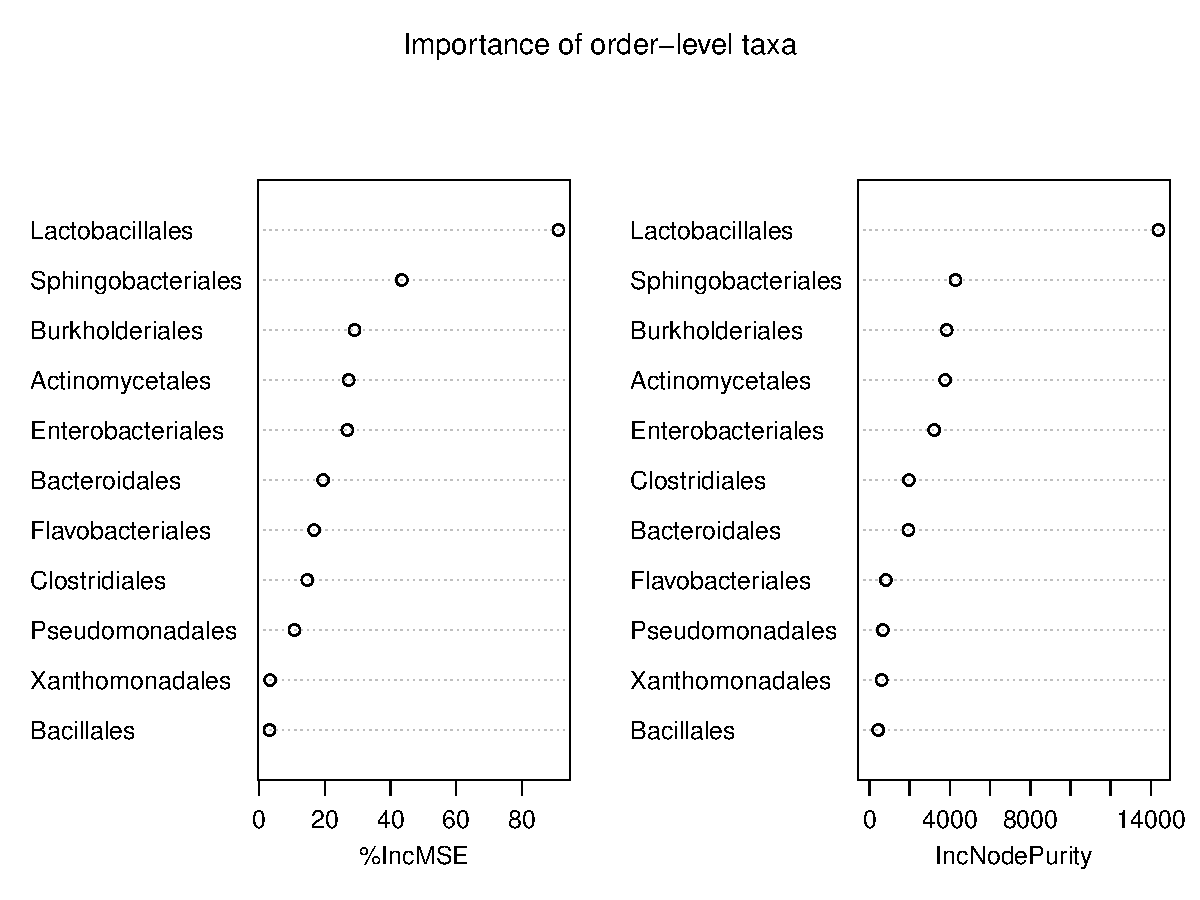
\includegraphics[width=3.25in]{orders_imp_plot}
\end{figure}
\end{center}
\vspace{-0.25in}
\noindent {\scriptsize The most important variable in determining the order-level taxa was Lactobacillales.  The fitted model was able to explain about 67.5\% of the variability, with a root MSE of about 11.3 days.  From cross-validation, the most reasonable models considered 6-8 splits and used at least 3000 ensemble trees.}

\end{frame}




\begin{frame}{Fitting the family taxa}

\begin{center}
\begin{figure}
  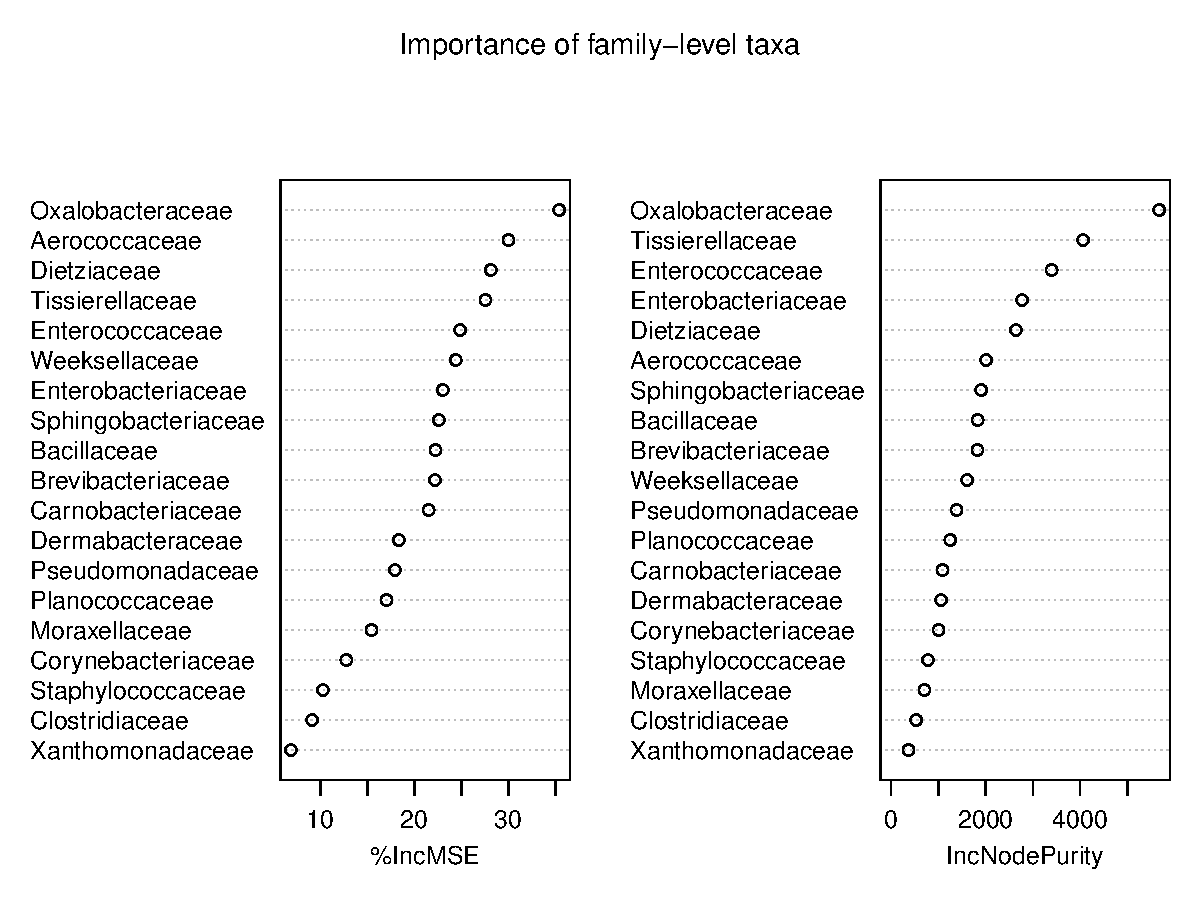
\includegraphics[width=3.25in]{families_imp_plot}
\end{figure}
\end{center}
\vspace{-0.25in}

\noindent {\scriptsize The most important variable in determining the
  order-level taxa was Oxalobacteraceae.  The fitted model was able to
  explain about 79.5\% of the variability, with a root MSE of about 9
  days.  From cross-validation, the most reasonable models considered
  4 splits and used about 3000 ensemble trees.}

\end{frame}




\begin{frame}{Fitting the phyla taxa}

\begin{center}
\begin{figure}
  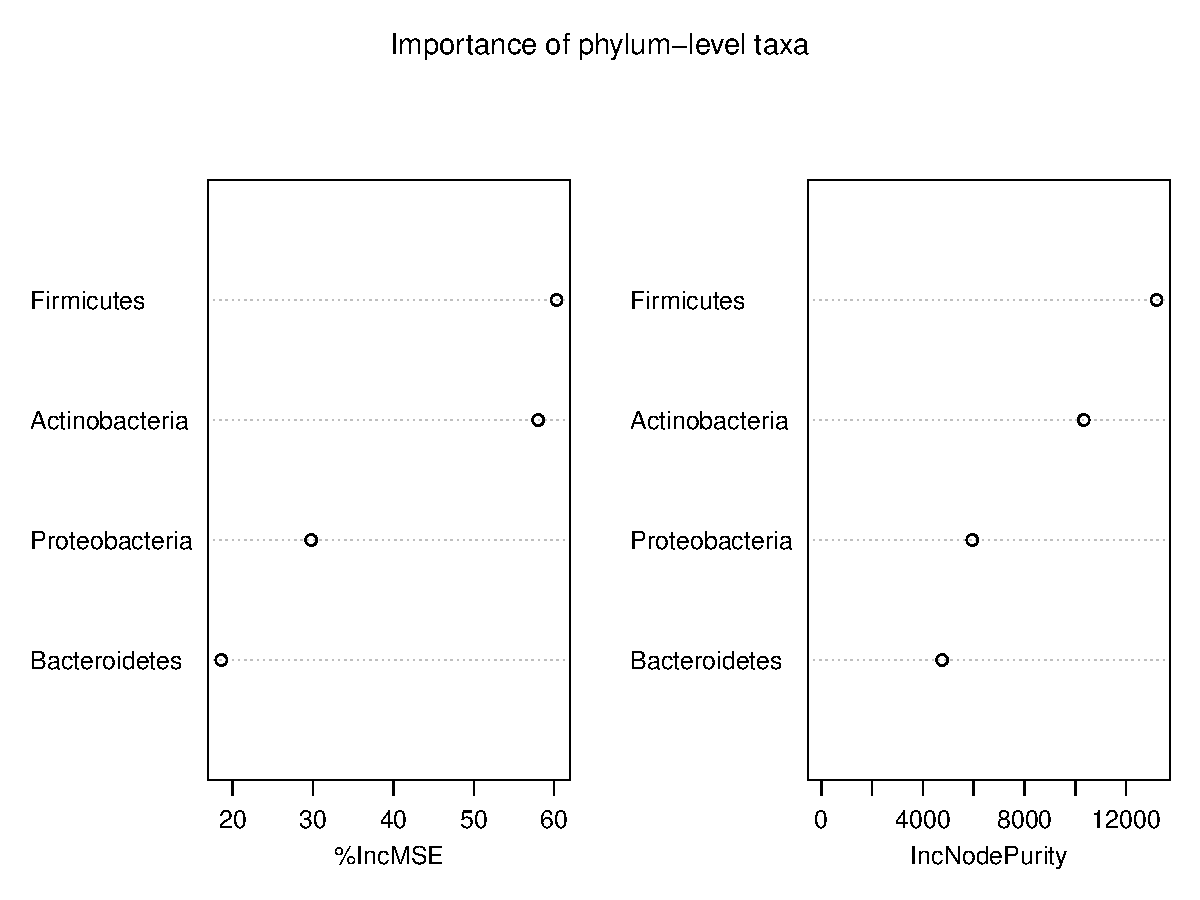
\includegraphics[width=3.25in]{phyla_imp_plot}
\end{figure}
\end{center}
\vspace{-0.25in}

\noindent {\scriptsize The most important variable in determining the
  order-level taxa was Firmicutes.  The fitted model was able to
  explain about 39.3\% of the variability, with a root MSE of about 15.5
  days.  From cross-validation, the most reasonable models considered
  2 splits and used about 3000 ensemble trees.}

\end{frame}




\begin{frame}{More discussion}
  
  \begin{itemize}
  \item The ``more specific'' the taxa-level, the smaller our
    mean-square error.  This is interesting, because as we get more
    specific, we have more unclassified material.  The unclassified
    material is excluded from the analysis.  So, even with the loss of
    that data, our predictions are still better with the family-level taxa.
  \item Random forest models are not easy to explain, as they do not produce a fitted regression line, etc.  However, it should be straightforward to make predictions when given a new dataset.
    \item It would be great to get some additional data to use to test
      these models.
  \item For now, I've put the PCA/GAM model idea on the back shelf, due
  to the difficulties in interpreting the effect of any one taxa when
  we use principal components.
\end{itemize}

\end{frame}



\end{document}
